\documentclass{article}
\usepackage{tikz, comment}
\usepackage{pifont}
\usepackage{fontspec, pgfplots}
\usetikzlibrary{arrows, decorations.markings, decorations.pathreplacing}
\begin{comment}
:Title: Not defined yet
:Tags: circumcenter;point of division formula;point of symmetry;pappus&#146;s theorem, theorem of pappus;origin
:Prob: 0.482;0.4738;0.4245;0.3969;0.3941
:Author: Prof.Hu Ji-shan, HKUST
:Slug: No name yet

Description Here.........
\end{comment}
\begin{document}\centering 

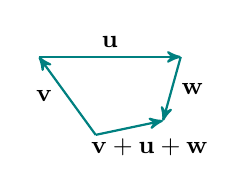
\begin{tikzpicture}[>=latex,xscale=.5*1.8, yscale=.5*1.8][font=\sf\small] 

\draw[teal, thick, ->, >=stealth'] (0, 0) -- (-0.8, 1.1)node[black, left, midway, pos=0.5, xshift=-2, yshift=0, scale=1]{$\bf v$}; %v

\begin{scope}[xshift=-0.8cm,yshift=1.1cm]
\draw[teal, thick, ->, >=stealth'] (0, 0) -- (2, 0)node[black, above, midway, pos=0.5, xshift=0, yshift=0, scale=1]{$\bf u$}; %u

\begin{scope}[xshift=2cm,yshift=0cm]
\draw[teal, thick, ->, >=stealth'] (0, 0) -- (-0.25, -0.9)node[black, right, midway, pos=0.5, xshift=0, yshift=0, scale=1]{$\bf w$}; %w
\end{scope}

\end{scope}

\draw[teal, thick, ->, >=stealth'] (0, 0) -- ({2-0.8-0.25}, {1.1+0-0.9})node[black, below, midway, pos=0.8, xshift=0, yshift=-2, scale=1]{$\bf v + u + w$};

\end{tikzpicture}
\end{document}